\subsection{ARFI Imaging}
Experimental ARFI imaging data were acquired using a modified Siemens Acuson
SC2000\texttrademark~ultrasound scanner (Siemens Healthcare, Ultrasound Business Unit,
Mountain View, CA, USA) and the longitudinal array of an Acuson ER7B
transducer.  The ARFI imaging sequence was comprised of
standard B-mode ultrasonic imaging, or tracking beams, and pushing beams. For
each lateral location, two pre-push reference images were acquired, then three
300 cycle pushing pulses were transmitted in rapid succession, focused at 30
mm, 22.5 mm, and 15 mm, respectively, and finally the response of the tissue
was tracked for up to 6ms at a PRF of 8kHz. This pushing strategy is similar to
what has been published by Bercoff \etal~\cite{Bercoff2004}. The 30 mm and 22.5
mm foci pushing pulses were transmitted at 4.6 MHz with a F/2 geometry and the
15 mm focus pushing pulse was transmitted at 5.4 MHz with a F/2.35 geometry to
maintain the same beamwidth (0.67 mm) throughout the region of excitation. A
total of 82 lateral locations were interrogated to cover the 55 mm field of
view, translating 0.67 mm laterally per location.

For the tracking pulses, 16 parallel receive lines at 5.0 MHz were spaced to
observe both the on and off-axis response of the tissue to the pushing pulses.
Specifically, four lines were dedicated to tracking the on-axis displacement,
with all 4 beams located inside the beamwidth of the pushing pulses such that
the beam spacing was 0.17 mm. 

3D volumetric imaging data was acquired using mechanical rotation of the ER7B
transducer between sequential imaging frames, sweeping across the lateral
extent of the prostate.  This rotation setup utilized a CIVCO
Micro-Touch\texttrademark stabalizer (CIVCO Medical Solutions, Kalona, IA USA)
that allows for complete 6-axis degrees of freedom for manual positioning of
the transducer to sweep through the entire prostate during imaging.  Sequential
imaging frames were $\sim$1\degree apart, depending on the absolute size of the
prostate.  A custom optical angular feedback transduction circuit utilizing a
reflective linear strip with 500 lines-per-inch (LPI) resolution (US Digital,
Vancouver, WA, USA) was coupled with a 141 oz-in torque stepper motor with
planetary gearbox (Model \#11YPG202S-LW4-R27, Anaheim Automation, Anaheim, CA,
USA) (Figure~\ref{fig:setup_annotated}) to achieve accurate spatial
localization of the imaging frames in the 3D dataset.

\begin{figure}
\centering
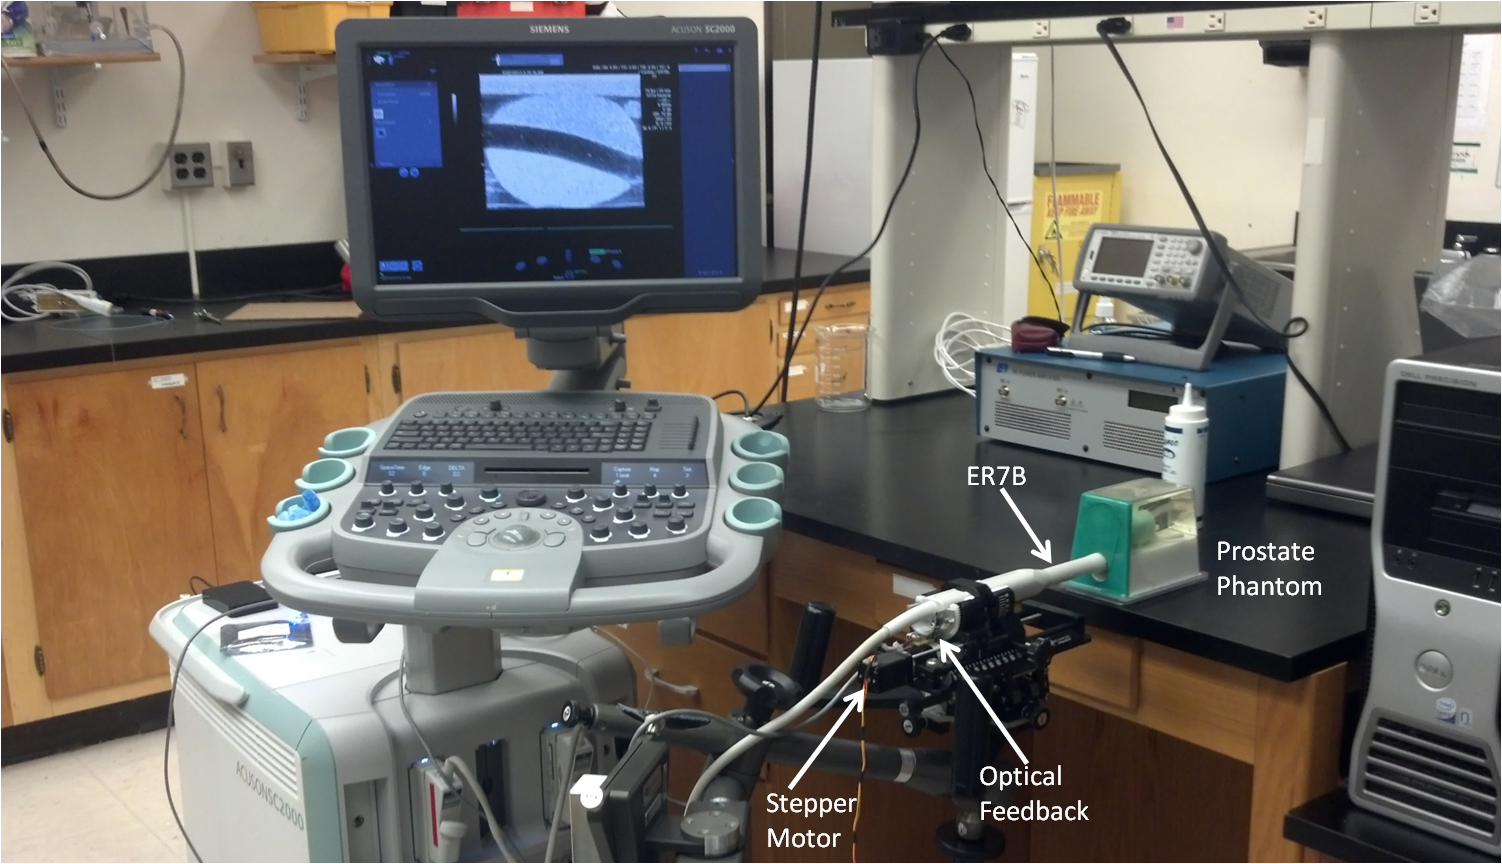
\includegraphics[width=0.75\textwidth]{figs/setup_annotated.png}
\caption{The experimental setup used for \textbf{B-mode/}ARFI imaging in the
    operating suite, including the Siemens SC2000 scanner with the ER7B
    endorectal transducer sitting in a custom cradle of a CIVCO
    Micro-Touch\texttrademark stabilizer with optical feedback controlling a
    stepper motor to acquire 3D ultrasound imaging data \invivo.
    Custom-written Python code was run on the scanner to trigger B-mode and
    ARFI imaging acquisition sequences relative to completed rotation
    increments of $\sim$1\degree.}
\label{fig:setup_annotated} 
\end{figure}


Displacement estimation was performed using a phase-shift estimator on the
beamformed in-phase and quadrature (IQ) data~\cite{Loupas95,pinton06}. The ARFI
data were then normalized as a function of depth to account for attenuation and
focal gain effects.  This normalization was performed using a displacement
profile measured in a homogeneous tissue-mimicking phantom, which was applied
to all displacements in the entire data set at each time step, and then
low-pass filtered with a cutoff-frequency of 0.8 mm$^{-1}$.

The normalized displacement data were scan-converted using a Delaunay
triangulation method with XXXX commaind in Matlab (R2012b, XXXX).  The
scan-converted ARFI imaging data had a final voxel size of XX x XX x XX mm.
